% Primary: Aarushi's protocol and submitted Q3 results; completed by Yuchen.
% Add graphicx to the main preamble and upload person_b_learning_curve.png.
\section{Effect of training data size (10 points)}
\question{Q2.1 [4 points].}{Configuration and required results.}
We extended Aarushi's existing TF-IDF logistic regression study, keeping C=4, at most 2,000 iterations, the shared 8,000/2,000 split, stratified subsampling and seeds 0, 1 and 2. We added the required 5,000-row point and training AUROC. Values below are means across three subsets, except the complete 8,000-row pool, which is fitted once. Each vocabulary and IDF is fitted on its own training subset only. The submitted style-model curves remain supplementary reference results.

\begin{center}\begin{tabular}{@{}rrr@{}}
\toprule Training rows & Mean train AUROC & Mean validation AUROC \\ \midrule
500 & 1.000000 & 0.869945 \\
1,000 & 1.000000 & 0.896831 \\
2,000 & 1.000000 & 0.924322 \\
5,000 & 1.000000 & 0.943272 \\
8,000 & 1.000000 & 0.950644 \\
\bottomrule\end{tabular}\end{center}
{\small Three subsampling seeds; 8,000 uses one complete-pool fit. Full-pool train AUROC is 0.999999875 before rounding.}
\question{Q2.2 [3 points].}{Training and validation learning curves.}
\begin{center}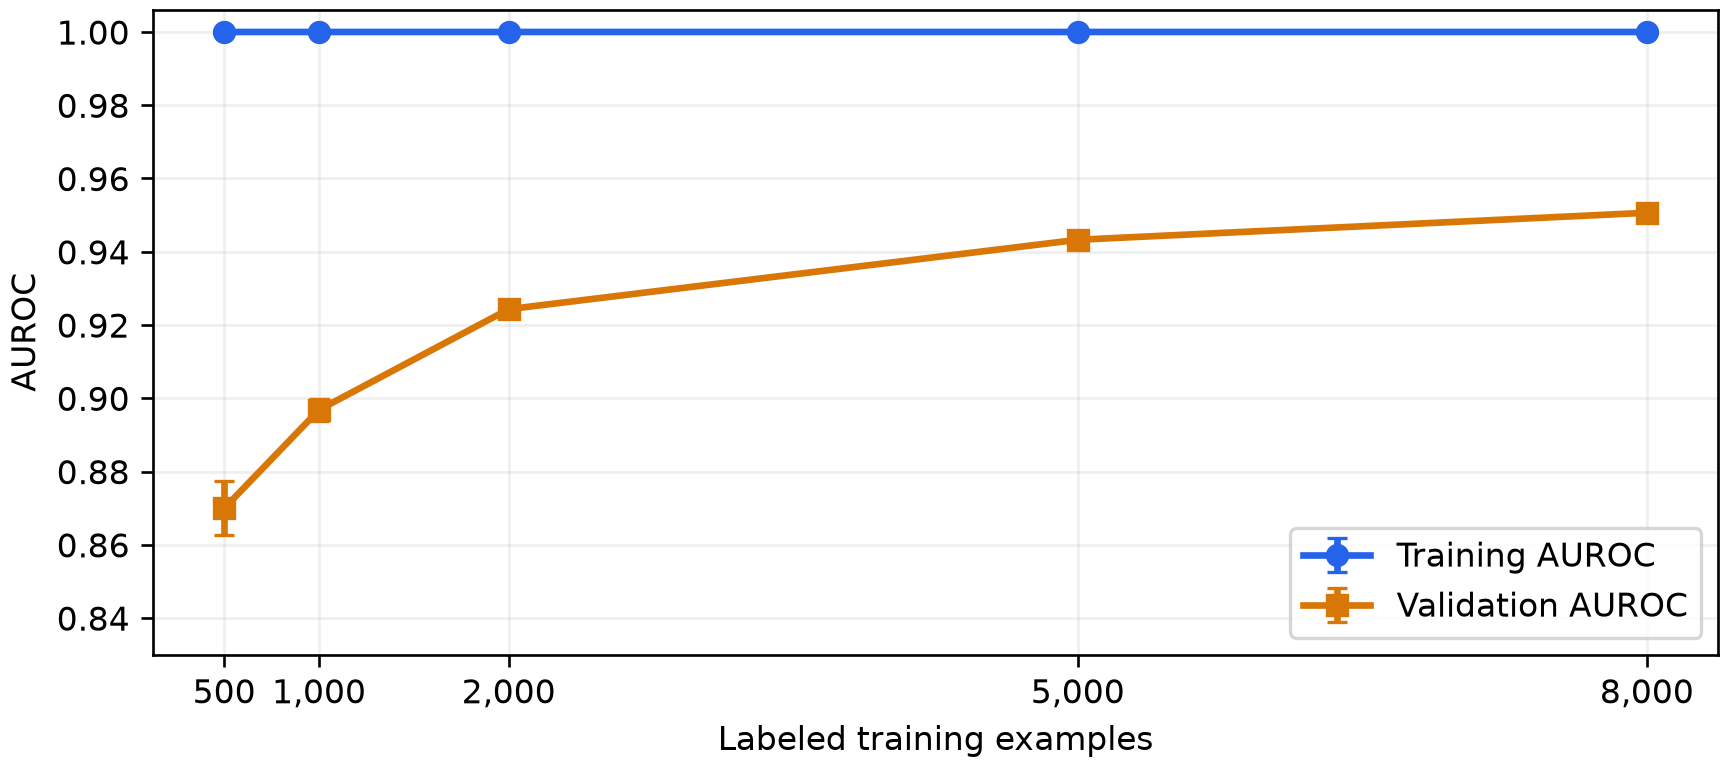
\includegraphics[width=0.96\linewidth]{person_b_learning_curve.png}\end{center}
\question{Q2.3 [3 points].}{Interpretation.}
Training AUROC remains essentially 1.0000 across all five training sizes, while mean validation AUROC increases from 0.8699 with 500 examples to 0.9506 with 8,000. This persistent gap suggests overfitting rather than clear underfitting. More labeled data reduces the gap and improves generalization on the fixed validation set. Gains diminish: increasing from 500 to 1,000 examples adds about 0.0269 AUROC, whereas adding 3,000 examples between 5,000 and 8,000 adds about 0.0074. Variation across the three sampling seeds is larger at small sizes. At 8,000, all seeds would use the same complete pool, so only one fit is reported. The trend supports more labels but does not establish performance beyond 8,000 or guarantee robustness under distribution shift.

\section{Learning from unlabeled data (5 points)}
\question{Q3.1 [2 points].}{Method and validation isolation.}
We used Aarushi's teacher-student pseudo-labeling method. A gradient boosting teacher on stylometric features and a TF-IDF logistic regression control were trained on the same 8,000 labeled examples. The teacher assigned labels to unlabeled passages when p(AI) was at least 0.95 or at most 0.05, retaining 2,612 examples. We then refitted the entire TF-IDF student, including vocabulary and IDF, on the augmented training set. Both models were scored on the unchanged 2,000-example validation set. Validation labels never entered fitting or pseudo-label generation. Three thresholds were explored on this fold; selecting 0.95 therefore provides exploratory evidence.

\question{Q3.2 [2 points].}{Primary submitted comparison.}
\begin{center}\begin{tabular}{@{}lrr@{}}
\toprule Method & Pseudo rows & Validation AUROC \\ \midrule
Supervised TF-IDF LR & 0 & 0.9506 \\
Style-teacher pseudo-labeling & 2,612 & 0.9537 \\
\bottomrule\end{tabular}\end{center}
{\small Source: Aarushi's unchanged submitted table; both use 8,000 true labeled rows. Values are reported to the four decimals available.}
\question{Q3.3 [1 point].}{Interpretation.}
Aarushi's style-teacher run improved validation AUROC from 0.9506 to 0.9537, approximately 0.0031. Self-training did not improve the control. A teacher with different features may contribute information the TF-IDF student misses. However, confidence does not guarantee correct labels, and the style model is sensitive to formatting artifacts. This setting was selected after comparing two teachers and three thresholds on the same validation fold, so its gain is exploratory. Our local repetition gave the same improvement direction but different style scores. We retain the original results as primary evidence and report the repetition separately, without claiming a statistically reliable benefit.

{\small Local replication selected 2,609 pseudo-labels and obtained 0.954365 versus 0.950644. It is preserved separately; small style-model discrepancies were not resolved to a single cause. Original inputs/split were unchanged.}
